\begin{dang}{Toán thực tế, liên môn về hàm số liên tục}
	Nội dung và phương pháp giải
\end{dang}
\Opensolutionfile{ans}[ans/ans-1K5-16-5]
\subsubsection{Ví dụ minh hoạ}
\setcounter{vd}{0}
\begin{vd}%[1K5BF-6]
	Tính $\underset{x\to +\infty}{\mathop{\lim}}\,\left( \sqrt{x^2+3x\sqrt{x}}-x+1 \right)$.
	\choice
	{\True $+\infty$}
	{$4$}
	{$-\infty$}
	{$\dfrac{1}{2}$}
	\loigiai{
		Có: $\underset{x\to +\infty}{\mathop{\lim}}\,\left( \sqrt{x^2+3x\sqrt{x}}-x+1 \right)=\underset{x\to +\infty}{\mathop{\lim}}\,\left( \dfrac{x^2+3x\sqrt{x}-x^2}{\sqrt{x^2+3x\sqrt{x}}+x}+1 \right)$\\
		$=\underset{x\to +\infty}{\mathop{\lim}}\,\left( \dfrac{3x\sqrt{x}}{\sqrt{x^2+3x\sqrt{x}}+x}+1 \right)$
		$=\underset{x\to +\infty}{\mathop{\lim}}\,\left(\sqrt{x} \dfrac{3}{\sqrt{1+3\sqrt{x}}+1}+1 \right)
		=+\infty$.}
\end{vd}



\begin{vd}%[1K5BF-6]
	Giới hạn hàm số $\underset{x\to -\infty}{\mathop{\lim}}\,\left(\sqrt{x^2-x\sqrt{|x|}+3}+x\right)$ bằng
	\choice
	{$0$}
	{$\dfrac{1}{2}$}
	{\True $+\infty$}
	{$-\infty $}
	\loigiai{
		Ta có
		$\underset{x\to -\infty}{\mathop{\lim}}\,\left(\sqrt{x^2-x\sqrt{|x|}+3}+x\right)$
		$=\underset{x\to -\infty}{\mathop{\lim}}\,\dfrac{\left(\sqrt{x^2-x\sqrt{|x|}+3}+x\right)\left(\sqrt{x^2-x\sqrt{|x|}+3}-x\right)}{\sqrt{x^2-x\sqrt{|x|}+3}-x}$\\
		$=\underset{x\to -\infty}{\mathop{\lim}}\,\dfrac{-x\sqrt{|x|}+3}{\sqrt{x^2-x\sqrt{|x|}+3}-x}$
		$=\underset{x\to -\infty}{\mathop{\lim}}\,\sqrt{|x|}\dfrac{-1+\dfrac{3}{x\sqrt{|x|}}}{-\sqrt{1-\sqrt{|x|}+\dfrac{3}{x^2}}-1}=+\infty$.}
\end{vd}
\begin{vd}%[1K5BF-6]
	Tìm giới hạn $I=\displaystyle\lim\limits_{x\to-\infty}\left(\sqrt{x^4+4x^3+1}-x^2\right)$
	\choice
	{$I=-4$}
	{$I=1$}
	{\True $I=-2$}
	{$I=-1$}
	\loigiai{
		Ta có \begin{eqnarray*}
			I&=&\displaystyle\lim\limits_{x\to-\infty}\left(\sqrt{x^4+4x^3+1}-x^2\right)=\displaystyle\lim\limits_{x\to-\infty}\dfrac{\left(\sqrt{x^4+4x^3+1}+x^2\right)\left(\sqrt{x^4+4x^3+1}-x^2\right)}{\sqrt{x^4+4x^3+1}+x^2}\\
			&=& \displaystyle\lim\limits_{x\to-\infty}\dfrac{4x^3+1}{\sqrt{x^4+4x^3+1}+x^2}=\displaystyle\lim\limits_{x\to-\infty}\dfrac{4x^3+1}{\sqrt{x^4+4x^3+1}+x^2}\\
			&=&\displaystyle\lim\limits_{x\to-\infty}x\dfrac{4+\dfrac{1}{x^3}}{\sqrt{1+\dfrac{4}{x}+\dfrac{1}{x^4}}+1}=-\infty.
		\end{eqnarray*}
	}
\end{vd}
\begin{vd}%[1K5BF-6]
	Tính $L=\lim\limits_{x \to - \infty} \left( \sqrt{x^2 -7x\sqrt{|x|}+1}- \sqrt{x^2-3x\sqrt{|x|}+2}\right)$.
	\choice
	{\True $L= + \infty$}
	{$L= - \infty$}
	{\True $L= 2$}
	{$L= -2$}
	\loigiai{
		\begin{align*}
			L &= \lim\limits_{x \to - \infty} \dfrac{-4x\sqrt{|x|}-1}{\sqrt{x^2 - 7x\sqrt{|x|} +1}+\sqrt{x^2-3x\sqrt{|x|}+2}}\\
			&=\lim\limits_{x \to - \infty} \dfrac{-4x\sqrt{|x|}-1}{-x \sqrt{1-\dfrac{7}{\sqrt{|x|}}+\dfrac{1}{x^2}}-x \sqrt{1-\dfrac{3}{\sqrt{|x|}}+\dfrac{2}{x^2}}}\\
			&= \lim\limits_{x \to - \infty}\sqrt{|x|} \dfrac{-4-\dfrac{1}{x\sqrt{|x|}}}{- \sqrt{1-\dfrac{7}{\sqrt{|x|}}+\dfrac{1}{x^2}}-\sqrt{1-\dfrac{3}{\sqrt{|x|}}+\dfrac{2}{x^2}}}\\
			&=+\infty.
		\end{align*}
	}
\end{vd}
\begin{vd}%[1K5BF-6]
	Tìm tham số m để $\displaystyle\lim\limits_{x\to +\infty}(\sqrt{{x^3+mx^2}}-x\sqrt{x})=-\infty$.
	\choice
	{$m=0$}
	{$m>0$}
	{\True $m<0$}
	{$m=2$}
	\loigiai{
		Ta có \begin{align*}
			\displaystyle \lim \limits_{x\to +\infty}\left (\sqrt{x^3+mx^2}-x\sqrt{x}\right ) =&\displaystyle \lim \limits_{x\to +\infty}\dfrac{mx^2}{\sqrt{x^3+mx^2}+x\sqrt{x}}\\
			=& \displaystyle \lim \limits_{x\to +\infty}\sqrt{x}\dfrac{m}{\sqrt{1+\dfrac{m}{x}} +1}.  
		\end{align*}	
		Do đó $\displaystyle\lim\limits_{x\to +\infty}(\sqrt{{x^3+mx^2}}-x\sqrt{x})=-\infty\Leftrightarrow m<0$.
	}
\end{vd}
\subsubsection{Bài tập rèn luyện}
\Opensolutionfile{ans}[ans/ans-1K5-2-Dang5]
\setcounter{ex}{0}
\begin{ex}%[1K5BF-6]
	Tính $\underset{x\to +\infty}{\mathop{\lim}}\,\left( \sqrt{x^2+3x\sqrt{x}}-x \right)$.
	\choice
	{\True $+\infty$}
	{$4$}
	{$-\infty$}
	{$\dfrac{1}{2}$}
	\loigiai{
		Ta có $\underset{x\to +\infty}{\mathop{\lim}}\,\left( \sqrt{x^2+3x\sqrt{x}}-x \right)=\underset{x\to +\infty}{\mathop{\lim}}\, \dfrac{x^2+3x\sqrt{x}-x^2}{\sqrt{x^2+3x\sqrt{x}}+x}$\\
		$=\underset{x\to +\infty}{\mathop{\lim}}\, \dfrac{3x\sqrt{x}}{\sqrt{x^2+3x\sqrt{x}}+x} $
		$=\underset{x\to +\infty}{\mathop{\lim}}\,\sqrt{x} \dfrac{3}{\sqrt{1+\dfrac{3}{x}}+1} 
		=+\infty$.}
\end{ex}
\begin{ex}%[1K5KF-6]
	$\lim \limits_{x\to -\infty} \left( \sqrt{4x^2+3x+1}+mx\right) = +\infty$ nếu
	\choice
	{\True $m<2$}
	{$m>2$}
	{$m\ge 2$}
	{$m\le 2$}
	\loigiai{
		Ta có 
		\[ \lim \limits_{x\to -\infty} \left( \sqrt{4x^2+3x+1}+mx\right) 
		= \lim \limits_{x\to -\infty}\left[ x\cdot \left( -\sqrt{4+\dfrac{3}{x}+\dfrac{1}{x^2}}+m\right) \right].\]
		Do $\lim \limits_{x\to -\infty} x = -\infty$ và $\lim \limits_{x\to -\infty} \left( -\sqrt{4+\dfrac{3}{x}+\dfrac{1}{x^2}}+m\right) = -2+m$ nên để \\ $\lim \limits_{x\to -\infty} \left( \sqrt{4x^2+3x+1}+mx\right) = +\infty$ thì $-2+m<0 \Leftrightarrow m<2$.
	}
\end{ex}


\begin{ex}%[1K5KF-6]
	Biết $\displaystyle \lim\limits_{x\to +\infty}\dfrac{(2-a)x-3}{x-\sqrt{{x^2+1}}}=+\infty $ (với $a$ là tham số). Giá trị nhỏ nhất của $P=a^2-2a+4$ là
	\choice
	{$3 $}
	{\True $4 $}
	{$5 $}
	{$1 $}
	\loigiai{
		Ta có $\displaystyle \lim\limits_{x\to +\infty}\dfrac{(2-a)x-3}{x-\sqrt{{x^2+1}}}=\displaystyle \lim\limits_{x\to +\infty}\dfrac{((2-a)x-3)\left(x+\sqrt{x^2+1}\right)}{x^2-x^2-1}=\displaystyle \lim\limits_{x\to +\infty} ((a-2)x+3)\left(x+\sqrt{x^2+1}\right)$
		\begin{itemize}
			\item Với $a=2$, $$\displaystyle \lim\limits_{x\to +\infty} ((a-2)x+3)\left(x+\sqrt{x^2+1}\right)=\displaystyle \lim\limits_{x\to +\infty} 3(x+\sqrt{x^2+1})=+\infty.$$
			\item Với $a>2$ suy ra $a-2>0$, nên $$\displaystyle \lim\limits_{x\to +\infty} ((a-2)x+3)\left(x+\sqrt{x^2+1}\right)=\displaystyle \lim\limits_{x\to +\infty} x\left((a-2)+\dfrac{3}{x}\right)\left(1+\sqrt{1+\dfrac{1}{x^2}}\right)=+\infty.$$
			\item Với $a<2$ suy ra $a-2<0$, nên $$\displaystyle \lim\limits_{x\to +\infty} ((a-2)x+3)\left(x+\sqrt{x^2+1}\right)=\displaystyle \lim\limits_{x\to +\infty} x\left((a-2)+\dfrac{3}{x}\right)\left(1+\sqrt{1+\dfrac{1}{x^2}}\right)=-\infty.$$
		\end{itemize}
		Vậy $a\ge 2$ thì $\displaystyle \lim\limits_{x\to +\infty}\dfrac{(2-a)x-3}{x-\sqrt{{x^2+1}}}=+\infty $.
		Xét hàm số $f(a)=a^2-2a+4$ với $a\ge 2$. Ta có bảng biến thiên sau
		\begin{center}
			\begin{tikzpicture}
				\tkzTabInit[nocadre=false, lgt=1.5, espcl=3]{$a$ /1,$f(a)$ /2}{$2$,$+\infty$}
				%\tkzTabLine{,-,$0$,+,}
				\tkzTabVar{-/ $4$,+/$+\infty $}
			\end{tikzpicture}
		\end{center}
		Suy ra $\min P=4$.
	}
\end{ex}
\begin{ex}%[1K5KF-6]
	Tìm số các số nguyên $m$ thỏa mãn $\displaystyle\lim\limits_{x\rightarrow +\infty} \left(3 \sqrt{mx^2+2x+1}-mx \right)= +\infty$.
	\choice
	{$4$}
	{$10$}
	{$3$}
	{\True $9$}
	\loigiai{
		\begin{itemize}
			\item Với $m=0$ thì $\displaystyle\lim\limits_{x\rightarrow +\infty} \left(3 \sqrt{2x+1} \right)= +\infty$ (thỏa yêu cầu bài toán).
			\item Với $m \neq 0$ ta có 
			$\displaystyle\lim\limits_{x\rightarrow +\infty} \left(3 \sqrt{mx^2+2x+1}-mx \right)= \lim\limits_{x\rightarrow +\infty} x\left(3 \sqrt{m+\dfrac{2}{x}+\dfrac{1}{x^2} }-m \right)= +\infty
			$.\\
			Suy ra 
			$\displaystyle\lim\limits_{x\rightarrow +\infty} \left(3 \sqrt{m+\dfrac{2}{x}+\dfrac{1}{x^2} }-m \right)= 3\sqrt{m}-m>0$, $(m>0)$.\\
			Ta có $3\sqrt{m}-m>0 \Leftrightarrow 3\sqrt{m}>m \Leftrightarrow m^2-9m<0 \Leftrightarrow 0<m<9$.	Do đó $m \in \{1;2;\ldots ;8\}$.
		\end{itemize}
		Vậy $m \in \{0;1;2;\ldots ;8\}$. 
	}
\end{ex}

\begin{ex}%[1K5KF-6]
	Giới hạn $\lim\limits_{x\to+\infty}\left(\sqrt{x^2-3x+1}+x\right)$ bằng
	\choice
	{\True $+\infty$}
	{$-\infty$}
	{$0$}
	{$2$}
	\loigiai{Ta có
		\begin{eqnarray*}
			&&\lim\limits_{x\to+\infty}\left(\sqrt{x^2-3x+1}+x\right)=\lim\limits_{x\to+\infty}\left(x\sqrt{1-\dfrac{3}{x}+\dfrac{1}{x^2}}+x\right)\\
			&=&\lim\limits_{x\to+\infty}\left(x\left(\sqrt{1-\dfrac{3}{x}+\dfrac{1}{x^2}}+1\right)\right)=+\infty.
		\end{eqnarray*}
		Vì $\lim\limits_{x\to+\infty}x=+\infty$ và $\lim\limits_{x\to+\infty}\left(\sqrt{1-\dfrac{3}{x}+\dfrac{1}{x^2}}+1\right)=2$.}
\end{ex}
\begin{ex}%[1K5KF-6]
	Biết $\displaystyle\lim_{x\rightarrow +\infty}\left(\sqrt{x^2+ax\sqrt{|x|}-1}-x\right)=-\infty$. Khi đó giá trị của tham số $a$ là
	\choice
	{\True $a<0$}
	{$a>0$}
	{$a=6$}
	{$a=10$}
	\loigiai{
		$\displaystyle\lim_{x\rightarrow +\infty}\left(\sqrt{x^2+ax\sqrt{|x|}-1}-x\right)=\lim_{x\rightarrow +\infty}\dfrac{x^2+ax\sqrt{|x|}-1-x^2}{\sqrt{x^2+ax\sqrt{|x|}-1}+x}=\lim_{x\rightarrow +\infty}\sqrt{|x|}\dfrac{a-\dfrac{1}{x\sqrt{|x|}}}{\sqrt{1+\dfrac{a}{\sqrt{|x|}}-\dfrac{1}{x^2}}+1}$.\\
		Để  $\displaystyle\lim_{x\rightarrow +\infty}\left(\sqrt{x^2+ax\sqrt{|x|}-1}-x\right)=-\infty\Leftrightarrow a<0$. 
	}
\end{ex}
\begin{ex}%[1K5KF-6]
	Tính $\displaystyle\lim_{x\rightarrow -\infty}\left(\sqrt{7x^2+2x\sqrt{|x|}}+x\sqrt{7}\right)$.
	\choice
	{$0$}
	{$-\dfrac{5\sqrt{7}}{14}$}
	{\True$-\infty$}
	{$+\infty$}
	\loigiai{$\displaystyle\lim_{x\rightarrow -\infty}\left(\sqrt{7x^2+2x\sqrt{|x|}}+x\sqrt{7}\right)=\lim_{x\rightarrow -\infty}\dfrac{2x\sqrt{|x|}}{\sqrt{7x^2+2x\sqrt{|x|}}-x\sqrt{7}}=\lim_{x\rightarrow -\infty}\dfrac{2x\sqrt{|x|}}{-x\sqrt{7+\dfrac2x}-x\sqrt{7}}\\=\lim_{x\rightarrow -\infty}\sqrt{|x|}\dfrac{2}{-\sqrt{7+\dfrac2x}-\sqrt{7}}=-\infty$.}
\end{ex}
\begin{ex}%[1K5KF-6]
	Cho số thực $a$ thỏa mãn $\lim\limits_{x\to -\infty}\left(\sqrt{x^4+5ax^3-1}-x^2\right)=-\infty$. Tìm số thực $a$.
	\choice
	{$(a<0$}
	{$a\in(-10;-5)$}
	{\True $a>0$}
	{$a\in(-3;-1)$}
	\loigiai{
		
		\begin{align*}
			\lim\limits_{x\to -\infty}\left(\sqrt{x^4+5ax^3-1}-x^2\right)
			&=\lim\limits_{x\to -\infty}\dfrac{x^4+5ax^3-1-x^4}{\sqrt{x^4+5ax^3-1}+x^2}\\
			&=\lim\limits_{x\to -\infty}x\dfrac{5a-\dfrac{1}{x^3}}{\sqrt{1+\dfrac{5a}{x}-\dfrac{1}{x^4}}+1}.
		\end{align*}
		Để $\lim\limits_{x\to -\infty}\left(\sqrt{x^4+5ax^3-1}-x^2\right)=-\infty\Leftrightarrow a>0.$
	}
\end{ex}
\begin{ex}%[1K5KF-6]
	Tính $\displaystyle \lim_{x\to+\infty}\left(3x^2+1-\sqrt{9x^4-6x^3+1}\right)$.
	\choice
	{$\dfrac{1}{4}$}
	{$\dfrac{1}{2}$}
	{\True $+\infty$}
	{$-\infty$}
	\loigiai{Vì $x\to+\infty$ nên ta có\\
		$$\begin{aligned}
			&\displaystyle \lim_{x\to+\infty}\left(3x^2+1-\sqrt{9x^4-6x^3+1}\right)\\
			=&\displaystyle \lim_{x\to+\infty} \dfrac{\left(3x^2+1-\sqrt{9x^4-6x^3+1}\right)\left(3x^2+1+\sqrt{9x^4-6x^3+1}\right)}{3x^2+1+\sqrt{9x^4-6x^3+1}}\\
			=&\displaystyle \lim_{x\to+\infty} \dfrac{\left(3x^2+1\right)^2-\left(9x^4-6x^3+1\right)}{3x^2+1+\sqrt{9x^4-6x^2+1}}\\
			=&\displaystyle \lim_{x\to+\infty} \dfrac{x^3\left(6+\dfrac{6}{x}\right)}{x^2\left(3+\dfrac{1}{x^2}+\sqrt{9-6\cdot\dfrac{1}{x^2}+\dfrac{1}{x^4}}\right)}\\
			=&\displaystyle \lim_{x\to+\infty} x\dfrac{6+\dfrac{6}{x}}{3+\dfrac{1}{x}+\sqrt{9-6\cdot\dfrac{1}{x}+\dfrac{1}{x^2}}}\\
			=&+\infty.
		\end{aligned}$$
	} 
\end{ex}
\begin{ex}%[1K5KF-6]
	Tính $\displaystyle \lim_{x\to+\infty}\left(2x-\sqrt{x^2-x+1}\right)$.
	\choice
	{\True $+\infty $}
	{$-\infty $}
	{$\dfrac{1}{2}$}
	{$-\dfrac{1}{2}$}
	\loigiai{Vì ${x\to +\infty}$ nên $\displaystyle \lim_{x\to+\infty}\left(2x-\sqrt{x^2-x+1}\right)=\displaystyle \lim_{x\to+\infty}x\cdot \displaystyle \lim_{x\to+\infty}\left(2-\sqrt{1-\dfrac{1}{x}+\dfrac{1}{x^2}}\right)=+\infty$.
	} 
\end{ex}
\begin{ex}%[1K5KF-6]
	Tìm giới hạn $M=\underset{x\to -\infty}{\lim}\left(\sqrt{x^2-4x\sqrt{|x|}}-\sqrt{x^2-x\sqrt{|x|}}\right)$.
	\choice
	{$M=-\infty$}
	{\True $M=+\infty$}
	{$M=-\dfrac{3}{2}$}
	{$M=\dfrac{1}{2}$}
	\loigiai{
		Ta có
		\begin{align*}
			M&=\underset{x\to -\infty}{\lim}\left(\sqrt{x^2-4x\sqrt{|x|}}-\sqrt{x^2-x\sqrt{|x|}}\right)\\
			&=\underset{x\to -\infty}{\lim}\dfrac{-3x\sqrt{|x|}}{\sqrt{x^2-4x\sqrt{|x|}}+\sqrt{x^2-x\sqrt{|x|}}}\\
			&=\underset{x\to -\infty}{\lim}\sqrt{|x|}\dfrac{-3}{-\sqrt{1-\dfrac{4}{\sqrt{|x|}}}-\sqrt{1-\dfrac{1}{\sqrt{|x|}}}}\\
			&=+\infty.
		\end{align*}
	}
\end{ex}


\begin{ex}%[1K5KF-6]
	Giá trị của $\lim \limits_{x \to  - \infty } \left( \sqrt {x^2 + 5}  - x \right)$ là
	\choice
	{\True $+\infty $}
	{$-\infty $}
	{$1$}
	{$0$}
	\loigiai{
		Ta có $$\lim\limits_{x \to -\infty} \left(\sqrt{x^2+5}-x\right)=\lim\limits_{x \to -\infty} x\left(-\sqrt{1+\dfrac{5}{x^2}}-1 \right)=+\infty.$$
	}
\end{ex}
\begin{ex}%[1K5KF-6]
	Giá trị của $\lim \limits_{x \to  + \infty } \left( \sqrt {x^2 + 5x\sqrt{x}}  - x \right)$ là
	\choice
	{\True $+\infty $}
	{$-\infty $}
	{$1$}
	{$0$}
	\loigiai{
		Ta có $$\lim\limits_{x \to +\infty} \left(\sqrt{x^2+5x\sqrt{x}}-x\right)=\lim\limits_{x \to +\infty} \dfrac{5x\sqrt{x}}{\sqrt{x^2+5x\sqrt{x}}+x}=\lim\limits_{x \to +\infty}\sqrt{x}\dfrac{5}{\sqrt{1+\dfrac{5}{\sqrt{x}}}+1}=+\infty.$$
	}
\end{ex}

\Closesolutionfile{ans}
